\documentclass[a4paper]{article}
\usepackage[spanish]{babel}
\usepackage[utf8]{inputenc}
\usepackage{charter}   % tipografia
\usepackage{graphicx}
\usepackage{wrapfig}
\usepackage[dvipsnames]{xcolor}
\usepackage{textcomp}
%\usepackage{makeidx}

%\usepackage{float}
%\usepackage{amsmath, amsthm, amssymb}
%\usepackage{amsfonts}
%\usepackage{sectsty}
%\usepackage{charter}
%\usepackage{wrapfig}
%\usepackage{listings}
%\lstset{language=C}

\usepackage{color} % para snipets de codigo coloreados
\usepackage{fancybox}  % para el sbox de los snipets de codigo

\definecolor{litegrey}{gray}{0.94}

% \newenvironment{sidebar}{%
% 	\begin{Sbox}\begin{minipage}{.85\textwidth}}%
% 	{\end{minipage}\end{Sbox}%
% 		\begin{center}\setlength{\fboxsep}{6pt}%
% 		\shadowbox{\TheSbox}\end{center}}
% \newenvironment{warning}{%
% 	\begin{Sbox}\begin{minipage}{.85\textwidth}\sffamily\lite\small\RaggedRight}%
% 	{\end{minipage}\end{Sbox}%
% 		\begin{center}\setlength{\fboxsep}{6pt}%
% 		\colorbox{litegrey}{\TheSbox}\end{center}}

\newenvironment{codesnippet}{%
	\begin{Sbox}\begin{minipage}{\textwidth}\sffamily\small}%
	{\end{minipage}\end{Sbox}%
		\begin{center}%
		\colorbox{litegrey}{\TheSbox}\end{center}}



\usepackage{fancyhdr}
\pagestyle{fancy}

%\renewcommand{\chaptermark}[1]{\markboth{#1}{}}
\renewcommand{\sectionmark}[1]{\markright{\thesection\ - #1}}

\fancyhf{}

%\fancyhead[LO]{Sección \rightmark} % \thesection\ 
\fancyfoot[LO]{\small{Ciruelos Rodríguez Gonzalo, Maddonni Axel, Thibeault Gabriel}}
\fancyfoot[RO]{\thepage}
\renewcommand{\headrulewidth}{0.5pt}
\renewcommand{\footrulewidth}{0.5pt}
\setlength{\hoffset}{-0.8in}
\setlength{\textwidth}{16cm}
%\setlength{\hoffset}{-1.1cm}
%\setlength{\textwidth}{16cm}
\setlength{\headsep}{0.5cm}
\setlength{\textheight}{25cm}
\setlength{\voffset}{-0.7in}
\setlength{\headwidth}{\textwidth}
\setlength{\headheight}{13.1pt}

\renewcommand{\baselinestretch}{1.1}  % line spacing


% \setcounter{secnumdepth}{2}
\usepackage{underscore}
\usepackage{caratula}
\usepackage{url}
\usepackage{float}


% ******************************************************** %
%              TEMPLATE DE INFORME ORGA2 v0.1              %
% ******************************************************** %
% ******************************************************** %
%                                                          %
% ALGUNOS PAQUETES REQUERIDOS (EN UBUNTU):                 %
% ========================================
%                                                          %
% texlive-latex-base                                       %
% texlive-latex-recommended                                %
% texlive-fonts-recommended                                %
% texlive-latex-extra?                                     %
% texlive-lang-spanish (en ubuntu 13.10)                   %
% ******************************************************** %
\usepackage{listings}


\renewcommand{\lstlistingname}{Codigo}
% Lenguajes soportados: ftp://ftp.tex.ac.uk/tex-archive/macros/latex/contrib/listings/listings.pdf
\lstloadlanguages{[ANSI]C} 
% FIXME: Me robe lo de abajo de otro ejemplo, estaba basado en Perl, ver si hay que cambiar algo
%\lstset{language=[x86masm]Assembler,
\lstset{language=[ANSI]C,
        frame=single,
        breaklines=true, 			% Saltar de linea si supero el maximo
        basicstyle=\small\ttfamily,
        keywordstyle=[1]\color{Blue}\bf,	% Color de las funciones de assembler
        keywordstyle=[2]\color{Purple},		% Color de parámetros especiales (registros, etc)
        identifierstyle=,                               
        commentstyle=\usefont{T1}{pcr}{m}{sl}\color{DarkGreen}\small,
        stringstyle=\color{Purple},     	% Strings purpuras
        showstringspaces=false,
        tabsize=4,
        %
        % Instrucciones no incluidas en el paquete Assembler
        morekeywords={global, define, section, .rodata, .text, jl, movd, movdqu, mulss, subss, addss, cmpss, pand, cvtss2si, cvttss2si, cvtsi2ss},
        %
        % Registros y esas otras cosas especiales que no son instrucciones
        morekeywords=[2]{rax,rdx,rcx,rbx,rsi,rdi,rsp,rbp,r8,r9,r10,r11,r12,r13,r14,r15,xmm0,xmm1,xmm2,xmm3,xmm4,xmm5,xmm6,xmm7
        		xmm8,xmm9,xmm10,xmm11,xmm12,xmm13,xmm14,xmm15,r8b, r9b, r10b, r11b, r8d, r9d, r10d, r11d},
       	%
        morecomment=[l][\color{Blue}]{...}, % Line continuation (...) like blue comment
        numbers=left, % Numeros de linea en la izquiera
        firstnumber=0, % Se arranca en la linea 1
        numberstyle=\tiny\color{Blue}, % Numeros de linea en azul y chicos
        stepnumber=0 % Los numerros de linea se muestran cada 5
}

\begin{document}

\thispagestyle{empty}
\materia{Organización del Computador II}
\submateria{Primer Cuatrimestre de 2015}
\titulo{Trabajo Práctico 3}
\subtitulo{System Programming - Tierra Pirata}
\grupo{Grupo Diablo II / PC}
\integrante{Ciruelos Rodríguez, Gonzalo}{063/14}{gonzalo.ciruelos@gmail.com} % obligatorio 
\integrante{Maddonni, Axel}{200/14}{axel.maddonni@gmail.com} % obligatorio 
\integrante{Thibeault, Gabriel}{}{} % obligatorio 

\maketitle
\newpage

\thispagestyle{empty}
\vfill

\thispagestyle{empty}
\vspace{3cm}
\tableofcontents
\newpage

%\normalsize
\newpage

\section{Introducción}

\newpage

\section{Desarrollo} 

\subsection{Ejercicio 1}

\textbf{Inicialización de la GDT}

Inicializamos la Tabla de Descriptores Globales con entradas para segmentos de código de nivel 0 y 3, otras para segmentos de datos de nivel 0 y 3, una para un segmento que describe el área de la pantalla de video, y la entrada correspondiente al segmento donde se guardará la tss de la tarea inicial. (Las entradas de gdt para las tss de las demás tareas son completadas al inicializarlas, como se explica en la sección correspondiente al Ejercicio 6).

\par Se utiliza desde el índice 8 por restricciones del trabajo práctico.
Los segmentos de datos y códigos están organizados de tal forma que se superpongan direccionando los primeros 500MB de memoria (Sistema FLAT), utilizando bloques de 4K al setear el bit de granularidad en 1.
\par Los demás atributos fueron seteados de la siguiente manera:
\par \textbf{\emph{Base y Límite: } }Como mencionamos anteriormente, los segmentos de código y datos están superpuestos. Comienzan en la dirección base 0x00000000, y el valor del límite 0x1F3FF corresponde la cantidad de bloques-1. Es decir, para cubrir 500MB se necesitan 128.000 bloques de 4K. El offset del último bloque es 127.999 (0x1F3FF en hexa).
Con respecto al segmento de video, éste ocupa en memoria desde la posición 0xB8000 hasta la 0xC0000, es decir 32K de memoria, cuyo máximo offset o límite es el correspondiente al último byte (7999 = 0x7FFF).
Para las tss, el límite es 0x68, pues miden 104 bytes cada una. Como base de la tarea inicial, seteamos la dirección 0x0000. ???????
\par \emph{\textbf{Tipo: }} El tipo para los segmentos de código es 0x0A (executable, readable), mientras que para los de datos y video es 0x02 (readable, writable).
\par \emph{\textbf{Sistema: }} El bit de system está seteado en 1 salvo en los segmentos correspondientes a las tss de las tareas, donde está activo bajo en 0 pues son potestad exclusiva del sistema operativo.
\par \emph{\textbf{DPL: }} Los segmentos de datos y código de nivel 0 tienen DPL en 0x00, al igual que los segmentos de sistema y el de video, mientras que los de código y datos nivel 3 tienen DPL en 0x03.
\par \emph{\textbf{Granularidad: }} El bit de G está activo sólo en los segmentos de datos y código ya que es necesario bloques de 4K para abarcar los 500MB.
\par \emph{\textbf{P, L, D/B, AVL: } }Seteados en 1, 0, 1 y 0 respectivamente para todas las entradas.
\newline

\textbf{Pasaje a Modo Protegido}

\par Para pasar a modo protegido, completamos y cargamos la GDT usando la instrucción lgdt, que toma el descriptor de la GDT con el tamaño y la dirección de la misma, habilitamos A20 para habilitar el acceso a direcciones superiores a los 2$^{20}$ bits, seteamos el bit de PE del registro CR0, y saltamos a 0x40:modoprotegido donde el 0x40 corresponde al Indice del segmento de código de nivel 0 (índice 8 en la gdt), corrido 3 ceros (estos ceros son los del TI y RPL).

\begin{lstlisting} [caption={Pasaje a modo protegido},label=modoproteg]
    
    ; Habilitar A20
    call habilitar_A20  
   
    ; Cargar la GDT
	lgdt [GDT_DESC]      ; cargo la estructura que esta en gdt.c

    ; Setear el bit PE del registro CR0
    mov eax, cr0
	or eax, 1
	mov cr0, eax

    ; Saltar a modo protegido
	jmp 0x40:modoprotegido

\end{lstlisting}

\newpage

\par Una vez trabajando en modo protegido, procedemos a establecer los selectores de segmentos de datos de nivel 0 (indice 9 en la gdt, corrido tres ceros correspondientes a los bits de TI y RPL), y el selector de segmento de video en fs (indice 12 en la gdt). Luego establecemos la base de la pila en la dirección 0x27000.


\begin{lstlisting} [caption={Pasaje a modo protegido},label=modoproteg2]
    modoprotegido:
    
    ; Establecer selectores de segmentos
    xor eax, eax
	mov ax,  1001000b
	mov ds, ax
	mov es, ax
	mov gs, ax
	mov ss, ax
    
	mov ax, 1100000b
    mov fs, ax

    ; Establecer la base de la pila
	mov ebp, 0x27000
	mov esp, 0x27000

\end{lstlisting}

\textbf{Inicialización de la Pantalla}

\par Para inicializar la pantalla llamamos a la función de screen.h \emph{screen_inicializar}, que se encarga de pintar la pantalla con el mapa, las barras para los jugadores, e inicializar los slots vacios y puntos en 0 de cada jugador, utilizando las funciones \emph{screen_pintar_rect} para pintar un rectangulo de color, \emph{print_dec} para imprimir los puntos, y \emph{screen_pintar} para imprimir caracteres.

\begin{figure}[ht!]
\centering
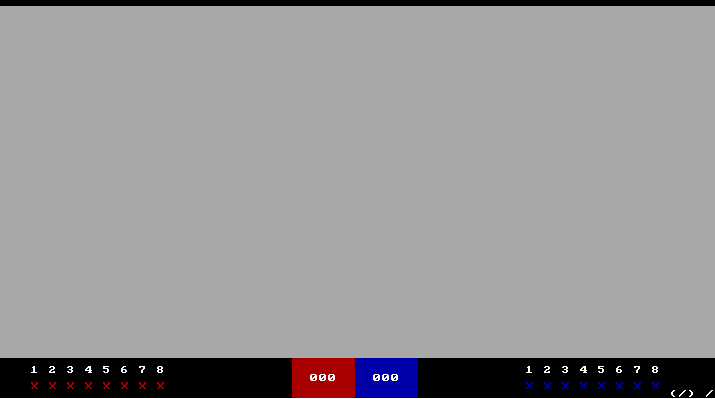
\includegraphics[width=120mm]{imagenes/pantalla.png}
\caption{Pantalla Inicial.}
\end{figure}

\subsection{Ejercicio 2}

\textbf{Inicialización de la IDT}

\par Para inicializar la IDT se llama a una funci\'on en lenguaje C, "void idt\_inicializar(void)". La IDT se representa mediante un arrelgo (de tama\~no 255) de "idt\_entry"
(esta estructura fue definida como lo muestra el extracto de C\'odigo \ref{idtEntry}, seg\'un las especificaciones dadas en el manual de Intel). Esta funci\'on utiliza un macro
(que se encuentra en el extracto de C\'odigo \ref{macro}) para inicializar cada una de las entradas necesarias de la IDT. 
\par El macro define el offset como los 16 bits menos y m\'as significativos (ya que \'este se encuentra separado en dos campos de 16 bits cada uno) de la direcci\'on de la tarea de atenci\'on
de la interrupci\'on correspondiente. El selector de segmento lo define como 0x0040, que es 0x8 (el indice del segmento de codigo de nivel de privilegio 0 en la GDT) shifteado 3 bits a la izquierda.
Los atributos los define como 0x8e00, que representan un segmento presente (P = 1), un nivel de privilegio de 0 (DPL = 00), un tama\~no de Gate de 32 bits (bits 8 a 12 de la Interrupt Gate = 0b01110),
y los 7 bits restantes en 0. 
\par La rutina de atenci\'on de cada interrupci\'on se genera a partir de un macro (que se encuentra en el extracto de C\'odigo \ref{macroISR}) que imprime el c\'odigo de error correspondiente
a pantalla y luego queda en un loop infinito.
\par La IDT ya inicializada se puede acceder tras ejecutar la instrucci\'on $lidt [IDT\_DESC]$. El descriptor de la IDT, "IDT\_DESC" es una estructura (definida como se ve en el extracto de
c\'odigo \ref{idtDesc}) que contiene el tama\~no de la IDT y su direcci\'on en memoria.

\begin{lstlisting} [caption={Estructura de idt\_entry},label=idtEntry]
typedef struct str_idt_entry_fld {
    unsigned short offset_0_15;
    unsigned short segsel;
    unsigned short attr;
    unsigned short offset_16_31;
} __attribute__((__packed__, aligned (8))) idt_entry;

\end{lstlisting}


\begin{lstlisting} [caption={Codigo del macro utilizado para inicializar la IDT},label=macro]
#define IDT_ENTRY(numero)                                                                                        
    idt[numero].offset_0_15 = (unsigned short) ((unsigned int)(&_isr ## numero) & (unsigned int) 0xFFFF);        
    idt[numero].segsel = (unsigned short) 0x0040;                                                                
    idt[numero].attr = (unsigned short) 0x8e00;                                                                  
    idt[numero].offset_16_31 = (unsigned short) ((unsigned int)(&_isr ## numero) >> 16 & (unsigned int) 0xFFFF);
\end{lstlisting}

\begin{lstlisting} [caption={Codigo del macro utilizado para la rutina de atencion de interrupciones},label=macroISR]
_isr%1:
    mov eax, %1
    push dword 0x0f0f 
    push dword 0
    push dword 0
    push MENSAJE_ERROR_%1
    call print
    
    jmp \$
\end{lstlisting}

\begin{lstlisting} [caption={Estructura de IDT\_Desc}],label=idtDesc] 
typedef struct str_idt_descriptor {
    unsigned short  idt_length;
    unsigned int    idt_addr;
} __attribute__((__packed__)) idt_descriptor;
\end{lstlisting}

\subsection{Ejercicio 3}

\par Para inicializar el directorio del kernel, lo que hacemos es, en la primera posicion declarar la tabla de kernel (que será identity mapping), y luego ponemos todo el resto de directorio en 0 (bit de presente en 0, que indica que esas entradas no direccionan nada).

\par Luego inicializamos la tabla de kernel, que está en identity mapping, como dijimos anteriormente. Eso es bastante fácil, ya que podemos usar la misma variable para iterar y para decir la dirección física a la que direccionará una dirección virtual.


\par Para pintar la pantalla usamos las funciones que nos permiten pintar rectángulos, que no necesitan explicación dado que son muy simples.

\subsection{Ejercicio 4}

\textbf{Inicialización de la MMU}

\par Para administrar la memoria en el área libre contamos con un contador de páginas inicializado en la dirección 0x00100000. A medida que el sistema necesita una página,  éste contador se incrementa en 4K, como muestra la siguiente implementación:

\begin{lstlisting} [caption={Contador de Páginas Libres}],label=mmucontador] 
void * siguiente_libre;

void inicializar_mmu()
{
  siguiente_libre = (void *) PAGE_COUNTER_INIT;
}

void * dar_siguiente()
{
    uint i;
    for(i = 0; i<1024; i++) ((pde *) siguiente_libre)[i].present = 0;
    siguiente_libre += 0x1000;
    return siguiente_libre - 0x1000;
}
\end{lstlisting}

\par Al crear una página, recorremos todas entradas de la tabla seteando el bit de presente en 0 (sea ésta un directorio o tabla de páginas). Para simplificar la manipulación en el código de las pde y pte creamos dos estructuras en C correspondientes a las ya mencionadas: 

\begin{lstlisting} [caption={struct Page Directory Entry}],label=mmupde] 
typedef struct pde_t {
    unsigned char present:1;
    unsigned char read_write:1;
    unsigned char user_supervisor:1;
    unsigned char page_level_write_through:1;
    unsigned char page_level_cache_disable:1;
    unsigned char accessed:1;
    unsigned char reserved:1;
    unsigned char page_size:1;
    unsigned char global:1;
    unsigned char available_9_11:3;
    unsigned int  base_address:20;
} __attribute__((__packed__, aligned (4))) pde;
\end{lstlisting}

\begin{lstlisting} [caption={struct Page Table Entry}],label=mmupte] 
typedef struct pte_t {
    unsigned char present:1;
    unsigned char read_write:1;
    unsigned char user_supervisor:1;
    unsigned char page_level_write_through:1;
    unsigned char page_level_cache_disable:1;
    unsigned char accessed:1;
    unsigned char dirty:1;
    unsigned char page_table_attribute_index:1;
    unsigned char global:1;
    unsigned char available_9_11:3;
    unsigned int  base_address:20;
} __attribute__((__packed__, aligned (4))) pte;
\end{lstlisting}

\textbf{Inicialización de directorios y tablas para Tareas Pirata}

\textbf{Mapeo y Desmapeo de Páginas}

\textbf{Testeo de Paginación (item no implementado en la sol final)}

\subsection{Ejercicio 5}

\textbf{Interrupción de Reloj}

\textbf{Interrupción de Teclado}

\textbf{Interrupción de sistema (0x46)}

\subsection{Ejercicio 6}

\subsection{Ejercicio 7}

 
\subsubsection*{Estructuras del scheduler}
 
La estructura en la que almacenamos los datos necesarios para la conmutación de tareas es muy simple. Básicamente son 3 datos

\begin{lstlisting}
struct {
  uint indiceA;
  uint indiceB;

  cual_t proximo;
} sched_struct;
\end{lstlisting}


\texttt{indiceA} nos indica cual es el próximo índice en el que deberíamos comenzar a buscar una nueva tarea para ejecutar del jugador A (similarmente \texttt{indiceB}). Notar que este índice puede corresponderse con una tarea válida del jugador tanto como con una tarea muerta o inválida.
 
\texttt{proximo}, nos indica a que jugador le toca jugar, es decir, en que arreglo de tareas vamos a comenzar nuestra búsqueda.
 
\subsubsection*{Algoritmos del scheduler}
 
La estructura que elegimos para el scheduler se ve fuertemente reflejada en los algorimos. Primero notemos como inicializamos las estructuras, todas en 0, y elegimos, arbitrariamente, que el proximo jugador al que le tocará es el A (podríamos haber elegido obviamente cualquiera).
 
Ahora inspeccionamos la funcion \texttt{sched_proxima_a_ejecutar}. Lo que hace es muy simple. 
Si el jugador al que le toca jugar es el A, comenzara buscando por su arreglo, desde \texttt{indiceA}, algún pirata que este vivo, y en caso de encontrarlo hara 4 cosas: setear a B como el proximo jugador, setear la id de la tarea actual con el id de la tarea seleccionada, inicializar mineros del jugador, si es que había mineros pendientes y finalmente devolver el indice en la gdt de la tss de la tarea seleccionada.
En caso de no encontrarlo, hará exactamente lo mismo con el arreglo del jugador B, buscando piratas vivos y etc.
 
\subsubsection*{Interrupción de reloj}
 
La última parte del scheduler que nos toca analizar es la parte que hace la conmutación de tareas, que es la interrupción de reloj.
 
La rutina de atención de interrupción de reloj es muy similar a la que nos dieron en clase. La única diferencia que tiene es que se fija si está activada la pantalla de debug, y en ese caso no hace nada (dado que no queremos que mientras la pantalla de debug esté activada, los piratas se sigan moviendo por el mapa).
 
El comportamiento del resto es realmente simple, llamamos a la función que nos da el indice de la gdt de la tss de la proxima tarea a ejecutar, la comparamos en el índice de la tarea actual (si la tarea es la misma no debemos saltar, porque saltaríamos a una tarea que tiene el bit de Busy en 1 y explota todo) y en caso de que sea distintos, saltamos.
 
Es importante notar que cuando se le reasigne la ejecución a una tarea, esta tarea va a volver a la linea que dice \texttt{popfd} y luego volverá a su ejecución común y corriente.
 
\subsubsection*{Modo Debug}
 
El modo debug es fácil de hacer una vez que el resto de las cosas están bien hechas. Debimos agregar un par de variables globales que nos indiquen si el modo debug está activado y otra que nos indique si se está mostrando la pantalla de debug en un momento dado.
 
Cuando nos llega una interrupción de las primeras 20, lo que hacemos es guardar toda la información que este disponible en ese momento (la que debemos guardar) y luego llamar a \texttt{game_pirata_exploto}.
 
En \texttt{game_pirata_exploto} (ademas de hacer las limpiezas de estructuras que correspondan) lo que hacemos es chequ si está el modo debug activado o no. En caso afirmativo, cargamos ciertas cosas que sean necesarias y llamamos a la función \texttt{screen_debug} que es realmente simple, muestra todos los datos en pantalla, mientras siga activado el modo debug. Cuando se vuelve a apretar 'y', el modo debug se desactiva y se sale de el loop, restaurando la pantalla como estaba (que previamente había sido backupeada).
 



\subsection{Ejercicio 8}

\newpage

\section{Conclusiones}

\end{document}

